 

% ----------------------------------------------------------------------
\section{CSM Model Description} \label{chap:model}


% .......................................................................
\subsection{Functional Objectives} \label{sec:ceil}

The European Train Control System ETCS relies on the existence of an
onboard controller in train engines, the \emph{European Vital Computer
  EVC}. Its functionality and basic architectural features are
described in the public ETCS system specification~\cite{ETCS}.  One
functional category of the EVC covers aspects of speed and distance
monitoring, to accomplish the \emph{``\ldots supervision of the speed
  of the train versus its position, in order to assure that the train
  remains within the given speed and distance
  limits.''}~\cite[3.13.1.1]{ETCSSRS-Principles}. While displaying
actual and allowed speed to the train engine driver, the monitoring
functions automatically trigger the brakes in case of speed limit
violations.  Speed and distance monitoring is decomposed into three
sub-functions~\cite[3.13.10.1.2]{ETCSSRS-Principles}, where only one
out of these three is active at a point in time: (1) \emph{Ceiling
  speed monitoring (CSM)} supervises the observance of the maximal
speed allowed according to the current most restrictive speed profile
(MRSP)\footnote{In some situations, more than one speed restriction
  may apply, and then the most restrictive one has to be enforced.}.
CSM is active while the train does not approach a target (train
station, level crossing, or any other point that must be reached with
predefined speed). (2) \emph{Target speed monitoring (TSM)} enforces
speed restrictions applicable while the train brakes to a target, for
example, a track section where a significantly lower maximal speed has
to be observed.  (3) \emph{Release speed monitoring (RSM)} applies
when the special target ``end of movement authority (EOA)'' is
approached, where the train must come to a stop. RSM supervises the
observance of the distance-depending so-called release speed, when the
train approaches the EOA and is allowed to drive at a reduced speed.

The model presented here captures the CSM functionality.



% .......................................................................
\subsection{System Requirements}
\label{sec:sysreq}
The ETCS system specification~\cite{ETCSSRS-Principles} defines the 11
following requirements for the CSM (see Table \ref{tab:req}). For
traceability purpose, The requirement identifiers refer to the
sections of the ETCS specification~\cite{ETCSSRS-Principles}. The
requirements are decomposed into two parts: the general requirements
that concern all the three supervision functions (including the CSM)
and the ones that only concern the CSM function.

%% Requirement REQ-3.13.10.3.3 is described by two tables (see
%% Table~\ref{tab:five} and Table~\ref{tab:six}), it is then
%% decomposed into sub-requirements REQ-3.13.10.3.3.t1, \ldots,
%% REQ-3.13.10.3.3.r1, each of them representing one line of these two
%% tables. 
%% Requirement REQ-3.13.10.3.4 is  represented as a transition table, it
%% is also decomposed into sub-requirements REQ-3.13.10.3.3.r1c2 to
%% REQ-3.13.10.3.3.r5c4 , one for each relevant cell of the table (see
%% Table~\ref{tab:seven}). For example the transition from {\sf Normal}
%% to {\sf Overspeed} corresponds to the requirement labeled
%% REQ-3.13.10.3.3.r3c1 (line 3, column 1).
%% In total we are dealing with \numreq{} requirements for the ceiling speed
%% monitoring specification.
   
% \begin{table}

{\tabsize
\renewcommand{\arraystretch}{1.2}

\begin{longtable}{lp{.7\textwidth}}
\caption{Requirements for the ceiling speed monitoring function
  (quoted verbatim
  from~\cite[3.13.10]{ETCSSRS-Principles}).\label{tab:req}}\\
\hline\hline
{\bf id} & {\bf Description}
\\\hline
\multicolumn{2}{c}{{\bf General Requirements}}\\\hline
REQ-3.13.10.2.1 & The train speed indicated to the driver shall be identical to the speed used for the speed monitoring. This shall be the estimated speed.
%%% (i.e. the estimated speed $\vest$).
\\\hline
REQ-3.13.10.2.2 & Once a Train Interface command (traction cut-off, service brake or emergency brake) is triggered, the on-board shall apply it until its corresponding revocation condition is met.
\\\hline
REQ-3.13.10.2.3 &
If there is no on-board interface with the service brake or if the use of the service brake command is not allowed by a National Value (only in Target speed monitoring),whenever a service brake command is specified, the emergency brake command shall be triggered instead.
\\\hline
REQ-3.13.10.2.4 &
The emergency brake command, which is triggered instead of the service brake command when an SBI supervision limit is exceeded, shall be revoked according to the requirements specified for the revocation of service brake command, unless the emergency brake command has been also triggered due to an EBI supervision limit. In such case, the condition for revoking the emergency brake command due to EBI supervision limit shall prevail.
\\\hline
REQ-3.13.10.2.5 &
The on-board shall revoke the Intervention status only when no brake command is applied by the speed and distance monitoring function.
\\\hline
\multicolumn{2}{c}{{\bf Requirements for CSM}}\\\hline
REQ-3.13.10.3.1&
The on-board equipment shall display the permitted speed.
%%% ($\vmax$).
\\\hline
REQ-3.13.10.3.2 &
When the supervision status is Overspeed, Warning or Intervention, the on-board equipment shall display the SBI speed.
%%% (i.e. the FLOI speed; FLOI = First Line of Intervention).
\\\hline
REQ-3.13.10.3.3&
The on-board shall compare the estimated speed with the ceiling
supervision limits defined in \cite[3.13.9.2]{ETCSSRS-Principles} and
shall trigger/revoke commands to the train interface (service brake if
implemented or emergency brake) and supervision statuses as described
in Table~\ref{tab:five} (from~\cite[Table~5]{ETCSSRS-Principles}) and
Table~\ref{tab:six} (from~\cite[Table~6]{ETCSSRS-Principles}).
\\\hline
REQ-3.13.10.3.4&
The on-board equipment shall execute the transitions between the different supervision statuses as described in Table~\ref{tab:seven} (see~\cite[4.6.1]{ETCSSRS-Principles} for details about the symbols). This table takes into account the order of precedence between the supervision statuses and the possible updates of the MRSP while in ceiling speed monitoring (e.g. when a TSR is revoked).
%%%; TSR = Temporary Speed Restriction).
\\\hline
REQ-3.13.10.3.5&
When the speed and distance monitoring function becomes active and the ceiling speed monitoring is the first one entered, the triggering condition t1 defined in Table~\ref{tab:five} shall be checked in order to determine whether the Normal status applies. If it is not the case, the on-board shall immediately set the supervision status to the relevant value, applying a transition from the Normal status according to Table~\ref{tab:seven}.
\\\hline
REQ-3.13.10.3.6&
The Indication status is not used in ceiling speed monitoring. However, in case the ceiling speed monitoring is entered and the supervision status was previously set to Indication, the on-board equipment shall immediately execute one of the transitions from the Indication status, as described in Table~\ref{tab:seven}.
\\
\hline\hline
\end{longtable}
}
 
\begin{table}[htbp]
\caption{Triggering of Train Interface commands and supervision statuses in ceiling speed monitoring (from~\cite[Table~5]{ETCSSRS-Principles}).}
\begin{center}
\tabsize
\begin{tabular}{lclcl}
\hline\hline
{\bf id} & {\bf TC} & {\bf Estimated speed} & {\bf TI} & {\bf SSE} 
\\\hline
REQ-3.13.10.3.3.t1 & t1 & $\vest \le \vmax$ & --- & Normal Status
\\
REQ-3.13.10.3.3.t2 & t2 & $\vest > \vmax$ & --- & Overspeed Status
\\
REQ-3.13.10.3.3.t3 & t3 & $\vest > \vmax + \dvw$ & --- & Warning Status
\\
REQ-3.13.10.3.3.t4 & t4 & $\vest > \vmax + \dvs$ & SB & Intervention Status
\\
REQ-3.13.10.3.3.t5 & t5 & $\vest > \vmax + \dve$ & EB & Intervention Status  
\\
\hline\hline
\end{tabular}
\end{center}

TC: trigger condition \newline
TI: command triggered on train interface to brakes \newline
SB: trigger service brake command (if available, otherwise trigger emergency brake)\newline
EB: trigger emergency brake command 
SSE: supervision status entered
\label{tab:five}
\end{table}%

 

\begin{table}[htbp]
\caption{Revocation of Train Interface commands and supervision
  statuses in ceiling speed monitoring
  (from~\cite[Table~6]{ETCSSRS-Principles}).}

\tabsize
\begin{minipage}{\textwidth}
\centering
\begin{tabular}{llcll}
\hline\hline
{\bf id} & {\bf RC} & {\bf Estimated Speed} & {\bf TICR} & {\bf SSR}
\\\hline
REQ-3.13.10.3.3.r0 & r0 & Standstill & EB & Intervention Status
\\
REQ-3.13.10.3.3.r1 & r1 & $\vest \le \vmax$ & SB  &
Indication Status \\
& & & EB$^*$ &
Overspeed Status\\
& & &  &
Warning Status \\
& & &  &
Intervention Status (if SBI) \\
& & &  &
Intervention Status (if EB$^*$ )\\
\hline\hline
\end{tabular}
\end{minipage}

$^*$ Only if $\areb = 1$.
\normalsize

RC: revocation condition \newline
TICR: command revoked on train interface to brakes \newline
SSR: supervision status revoked

\normalsize
\label{tab:six}
\end{table}%



\begin{table}[htbp]
\caption{Transitions between supervision statuses in ceiling speed
  monitoring (from~\cite[Table~7]{ETCSSRS-Principles}).}
\begin{center}
%\begin{tabular}{|p{20mm}|p{20mm}|p{20mm}|p{20mm}|p{20mm}|}
\begin{tabular}{|c|c|c|c|c|}
\hline
Normal  &   $< r1$ &   $< r1$ &   $< r1$ & $< r0,r1$
\\\hline
    &    Indication  & & & 
 \\\hline
    $t2 >$ &    $t2 > $ &   Overspeed  & & 
 \\\hline
    $t3 >$ &     $t3 >$ &    $t3 >$ &   Warning  &
 \\\hline
    $t4,t5 >$ &     $t4,t5 >$ &   $t4,t5 >$ &   $t4,t5 >$ &   Intervention
\\\hline
\end{tabular}
\end{center}


\smallskip
\footnotesize
 The
  sub-requirements IDs associated with each cell in the transition table
   are of the form  REQ-3.13.10.3.4.rXcY where X and Y
  are the row and   column indexes, respectively. 
\normalsize
\label{tab:seven}
\end{table}%

% .......................................................................
\subsection{Test Model Semantics}\label{sec:bsem} 
SysML test models are structured using blocks. At the top-level, the
model is decomposed into a block representing the system under test
(SUT) and another one representing the test environment (TE);
Fig.~\ref{fig:sysif} shows this decomposition for the CSM.  Depending
on the complexity of the model, blocks can be further decomposed into
lower-level block diagrams, until leaf blocks are reached that are
associated with behaviour. In our test models this behaviour is
specified by sequential hierarchic SysML state machines. Blocks
execute concurrently and in a synchronous way, so that transitions of
concurrent state machines that are enabled in the same model state
execute simultaneously.

The whole model executes according to the {\it run-to-completion}
semantics defined for state machines. The model is in a {\it
  quiescent} (or stable) state, if no transition can be executed
without an input change or time passing.

 
In a quiescent model state, inputs may be changed.  If these changes
enable a transition, the latter is executed. Our SUT model is
deterministic, this is typical for sequential safety-critical
applications, but note that possible occurrences of non-deterministic models in 
a safety-critical context are discussed in Section~\ref{sec:conc}.
Due to determinism, there is no necessity to handle situations where
several transitions are simultaneously enabled.  The executed
transition, however, may lead to a {\it transient} state, that is, to
a state where another transition is enabled. In the run-to-completion
semantics this new transition is also executed, and so forth until a
quiescent state is reached. Conceptually, the consecutive execution of
model transitions is executed in zero time, so that input changes
cannot happen until the next quiescent state has been reached.
Moreover, models admitting unbounded sequences of transitions between
transient states are considered as illegal, and this situation is
called a {\it livelock} failure.


% .......................................................................
\subsection{Interfaces}


The interfaces between SUT and its environment are specified in the
internal block diagram displayed in Fig.~\ref{fig:sysif}. All
interfaces are represented as flow ports. The environment writes to
SUT input ports and reads from SUT output ports.

\begin{figure}
 %%\hspace*{-40mm}
 \centering
 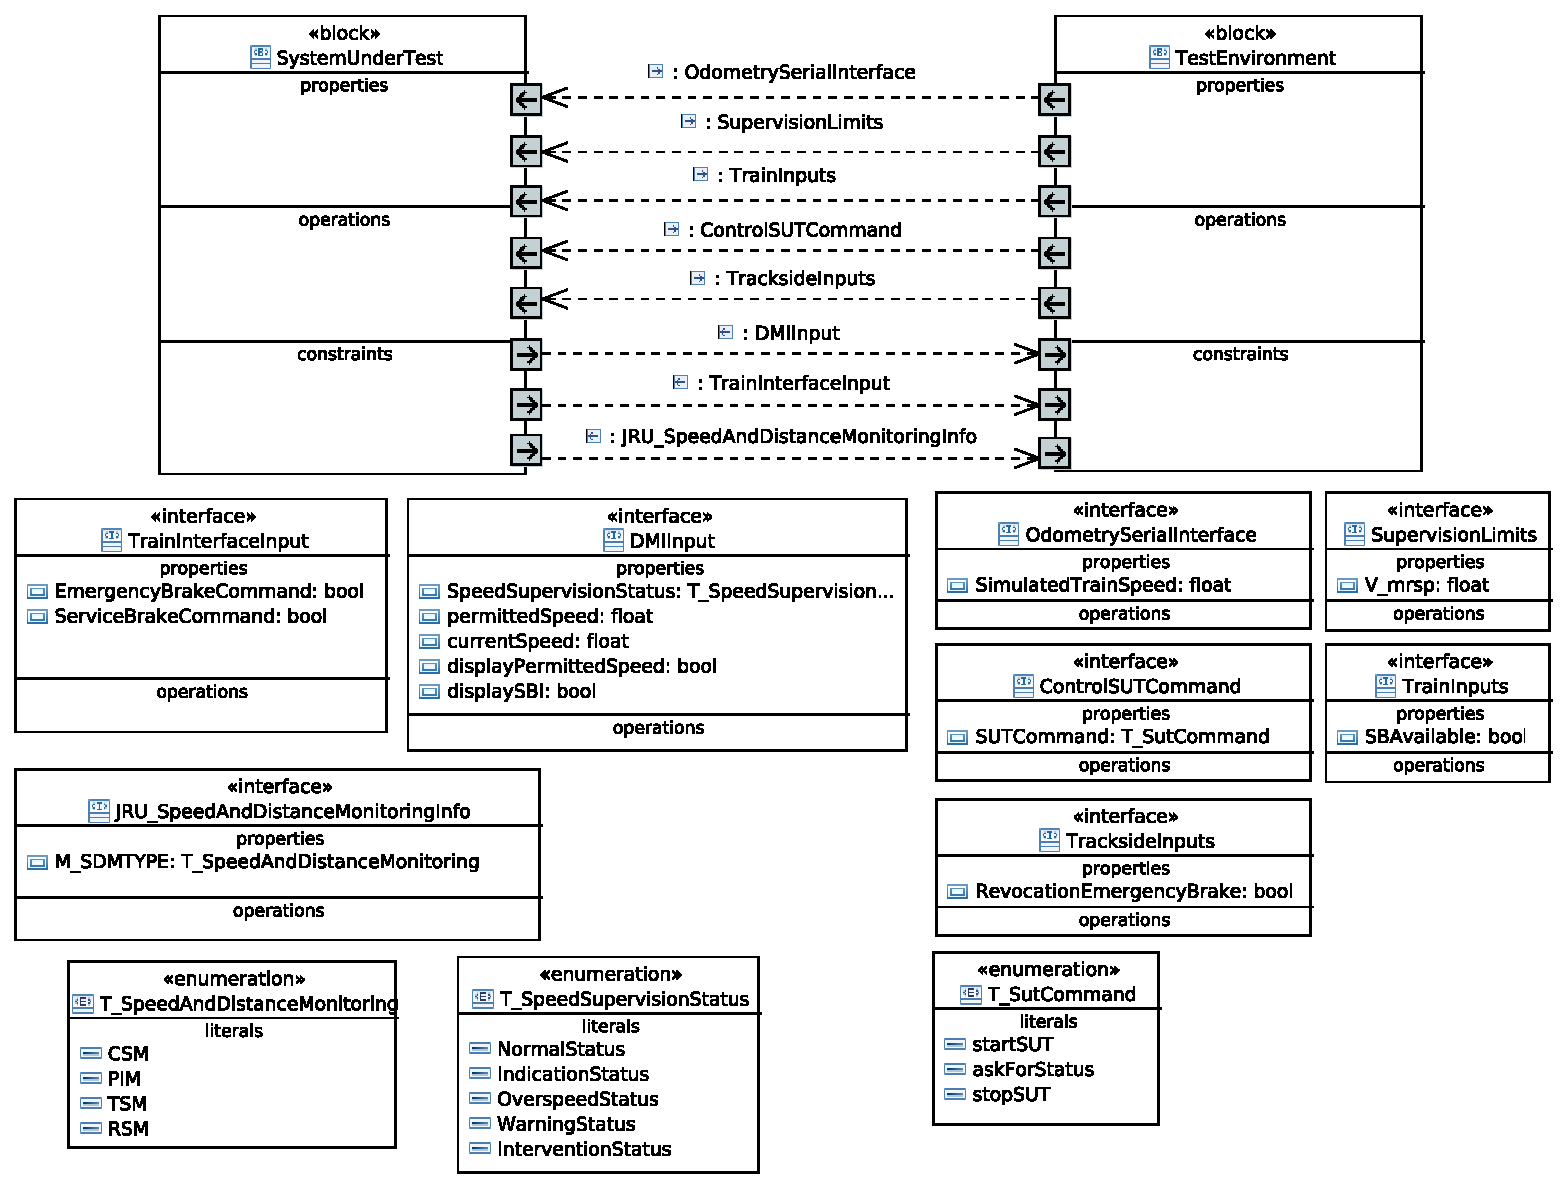
\includegraphics[width=\textwidth]{CSM-Interface.pdf} 
 %\vspace*{-5mm}
\caption{System interface of the ceiling speed monitor.}
 \label{fig:sysif}
 \end{figure}


 
Ceiling speed monitoring is activated and de-activated by the speed
and distance monitoring (SnD) coordination function that controls CSM,
TSM, and RSM: on input interface {\sf ControlSUTCommand}, variable $\csmsw$
specifies whether ceiling speed monitoring should be active
($\csmsw=\mathsf{startSUT}$) or passive, since target or release speed monitoring is
being performed ($\csmsw = \mathsf{stopSUT}$). 

The interface {\sf TrainInputs} carries
variable $\sbia$ which has value 1, if the train is equipped with a
service brake. This brake is then used for slowing down the train if
it has exceeded the maximal speed allowed, but not yet reached the
threshold for an emergency brake intervention. If $\sbia = 0$, the
emergency brake shall be used for slowing down the train in this
situation. Input $\sbia$ is to be considered as a configuration
parameter of the train, since it depends on the availability of the
service brake hardware. Therefore this value can be freely selected at
start-of-test, but must remain constant during test execution.

Input interface {\sf OdometrySerialInterface} provides the current
speed value estimated by the odometer equipment in variable
$\vest$. Input interface {\sf SupervisionLimits} provides the current
maximal velocity defined by the most restrictive speed profile in
variable $\vmax$. Input interface {\sf TracksideInput} provides a
control flag for the ceiling speed monitor: variable $\areb$ is 1, if
after an emergency brake intervention the brake may be automatically
released as soon as the estimated velocity of the train is again less
or equal to the maximal speed allowed. Otherwise ($\areb = 0$) the
emergency brakes must only be released after the train has come to a
standstill ($\vest = 0$).  This input parameter is a part of the
``national values'' given by the tracks, it may change when a train
crosses the boundaries between European countries, due to their local
regulations.

Output interface {\sf DMIInput} sends data from the SUT to the driver
machine interface (DMI). It carries five variables. $\dmicmd$ is used
to display the supervision status to the train engine driver: Value
{\sf IndicationStatus} may be initially present when CSM is activated,
but will be immediately overridden by one of the values {\sf
  NormalStatus}, {\sf OverspeedStatus}, {\sf WarningStatus}, or {\sf
  InterventionStatus}, as soon as ceiling speed monitoring becomes
active. Value {\sf NORMAL} is written by the SUT to this variable as long as
the ceiling speed is not violated by the current estimated
speed. Value {\sf OverspeedStatus} has to be set by the CSM as soon as
condition $\vmax < \vest$ becomes true. If the speed increases further
(the detailed conditions are described below), the indication changes
from {\sf OverspeedStatus} to {\sf WarningStatus}, and from there to
{\sf InterventionStatus}. The latter value indicates that either the
train is slowed down until it is back in the normal speed range, or
the emergency brake has been triggered to stop the train.
Furthermore, interface {\sf DMIInput} contains several speed-related
variables that are displayed on the DMI.





Output interface {\sf TrainInterfaceInput} specifies the train
interface from the CSM to the brakes, using variables $\ebcmd$ and
$\sbcmd$. If both equals $0$, both service
brakes (if existent) and emergency brakes are released. If $\sbcmd$ is
activated and $\ebcmd$ is not, the service brake is activated. If
$\ebcmd$ is activated, the emergency brake is
triggered.

Output interface {\sf JRU\_SpeedAndDistanceMoinitoringInfo} carries
the variable {\sf M\_SDMTYPE} that indicates which sub-function of the
speed and distance monitoring is active. 
The Juridical Recording Unit (JRU) is  used to record information
during the test phase, we have used this
interface as well as the DMI interface in compliance  with the testing
methodology defined by the European railway agency in \cite{ETCS-Subset076} (see section
\ref{sec:manualTest}).




% .......................................................................
\subsection{SUT Attributes and Operations}
The CSM executes sequentially; therefore 
the SUT block on the top-level interface diagram (Fig.~\ref{fig:sysif})  is refined 
to a single block representing the CSM,   as shown in Fig.~\ref{fig:sutcomposite}.
There, the SUT uses a local attribute $\sbicmd$ which 
carries value $1$, if the service
brake should be used for slowing down the train to the admissible
speed. If the value $0$ is assigned to 
$\sbicmd$, the emergency brake will be triggered in this situation.

\begin{figure}
%\hspace*{-50mm}
\centering
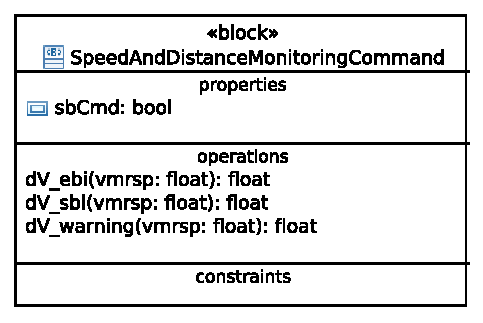
\includegraphics[]{CSM-SystemUnderTest.pdf}
%%\vspace*{-35mm}
\caption{Block diagram with CSM (sequential behaviour).}
 \label{fig:sutcomposite}
 \end{figure}


 
 
Three supervision limits are computed to assist the driver in
preventing automated service or emergency brake intervention by
maintaining the speed within certain limits, namely Warning, Service
brake intervention (sbi) and emergency brake intervention (ebi)
limits. These limits depend on the MRSP, and they are calculated
according to \cite{ETCSSRS-Principles} as follows.



 
\begin{equation}\label{eq:dvw}
\dvw(\vmax) = \left\{
\begin{array}{lc}
\min\{\frac{1}{3} + \frac{1}{30}\cdot\vmax,5 \}  &    \text{if}\ \ \vmax > 110 \\
4  &  \text{if}\ \ \vmax\le  110 \\
\end{array}
\right.
\end{equation}

\begin{equation}\label{eq:dvsbi}
\dvs(\vmax) = \left\{
\begin{array}{lc}
\min\{0.55+0.045\cdot\vmax,10 \}  &    \text{if}\ \ \vmax > 110 \\
5.5  &  \text{if}\ \ \vmax\le  110 \\
\end{array}
\right.
\end{equation}

\begin{equation}\label{eq:dvwe}
\dve(\vmax) = \left\{
\begin{array}{lc}
\min\{-0.75 + 0.075\cdot\vmax,15 \}  &    \text{if}\ \ \vmax > 110 \\
7.5  &  \text{if}\ \ \vmax\le  110 \\
\end{array}
\right.
\end{equation}

 


   
% .......................................................................
\subsection{CSM Behavioural Specification}
The behaviour of the ceiling speed monitor is modeled by a hierarchic state machine 
that is associated with the SUT block of Fig.~\ref{fig:sutcomposite}. The top-level machine (not shown here)
specifies the activation and de-activation of the CSM during the interplay between CSM, TSM, and RSM: state machine {\sf CSM\_ON} (this is the machine 
describing the behaviour of the CSM) is entered as soon as the value of 
input variable $\csmsw$ changes to {\sf startSUT}, and it is left when its value
changes to {\sf stopSUT}. 
The lower-level state machine  {\sf CSM\_ON}
models the behaviour of the active CSM, as displayed in Fig.~\ref{fig:csmsm}.

\begin{figure}
 \centering
%\hspace*{-15mm}
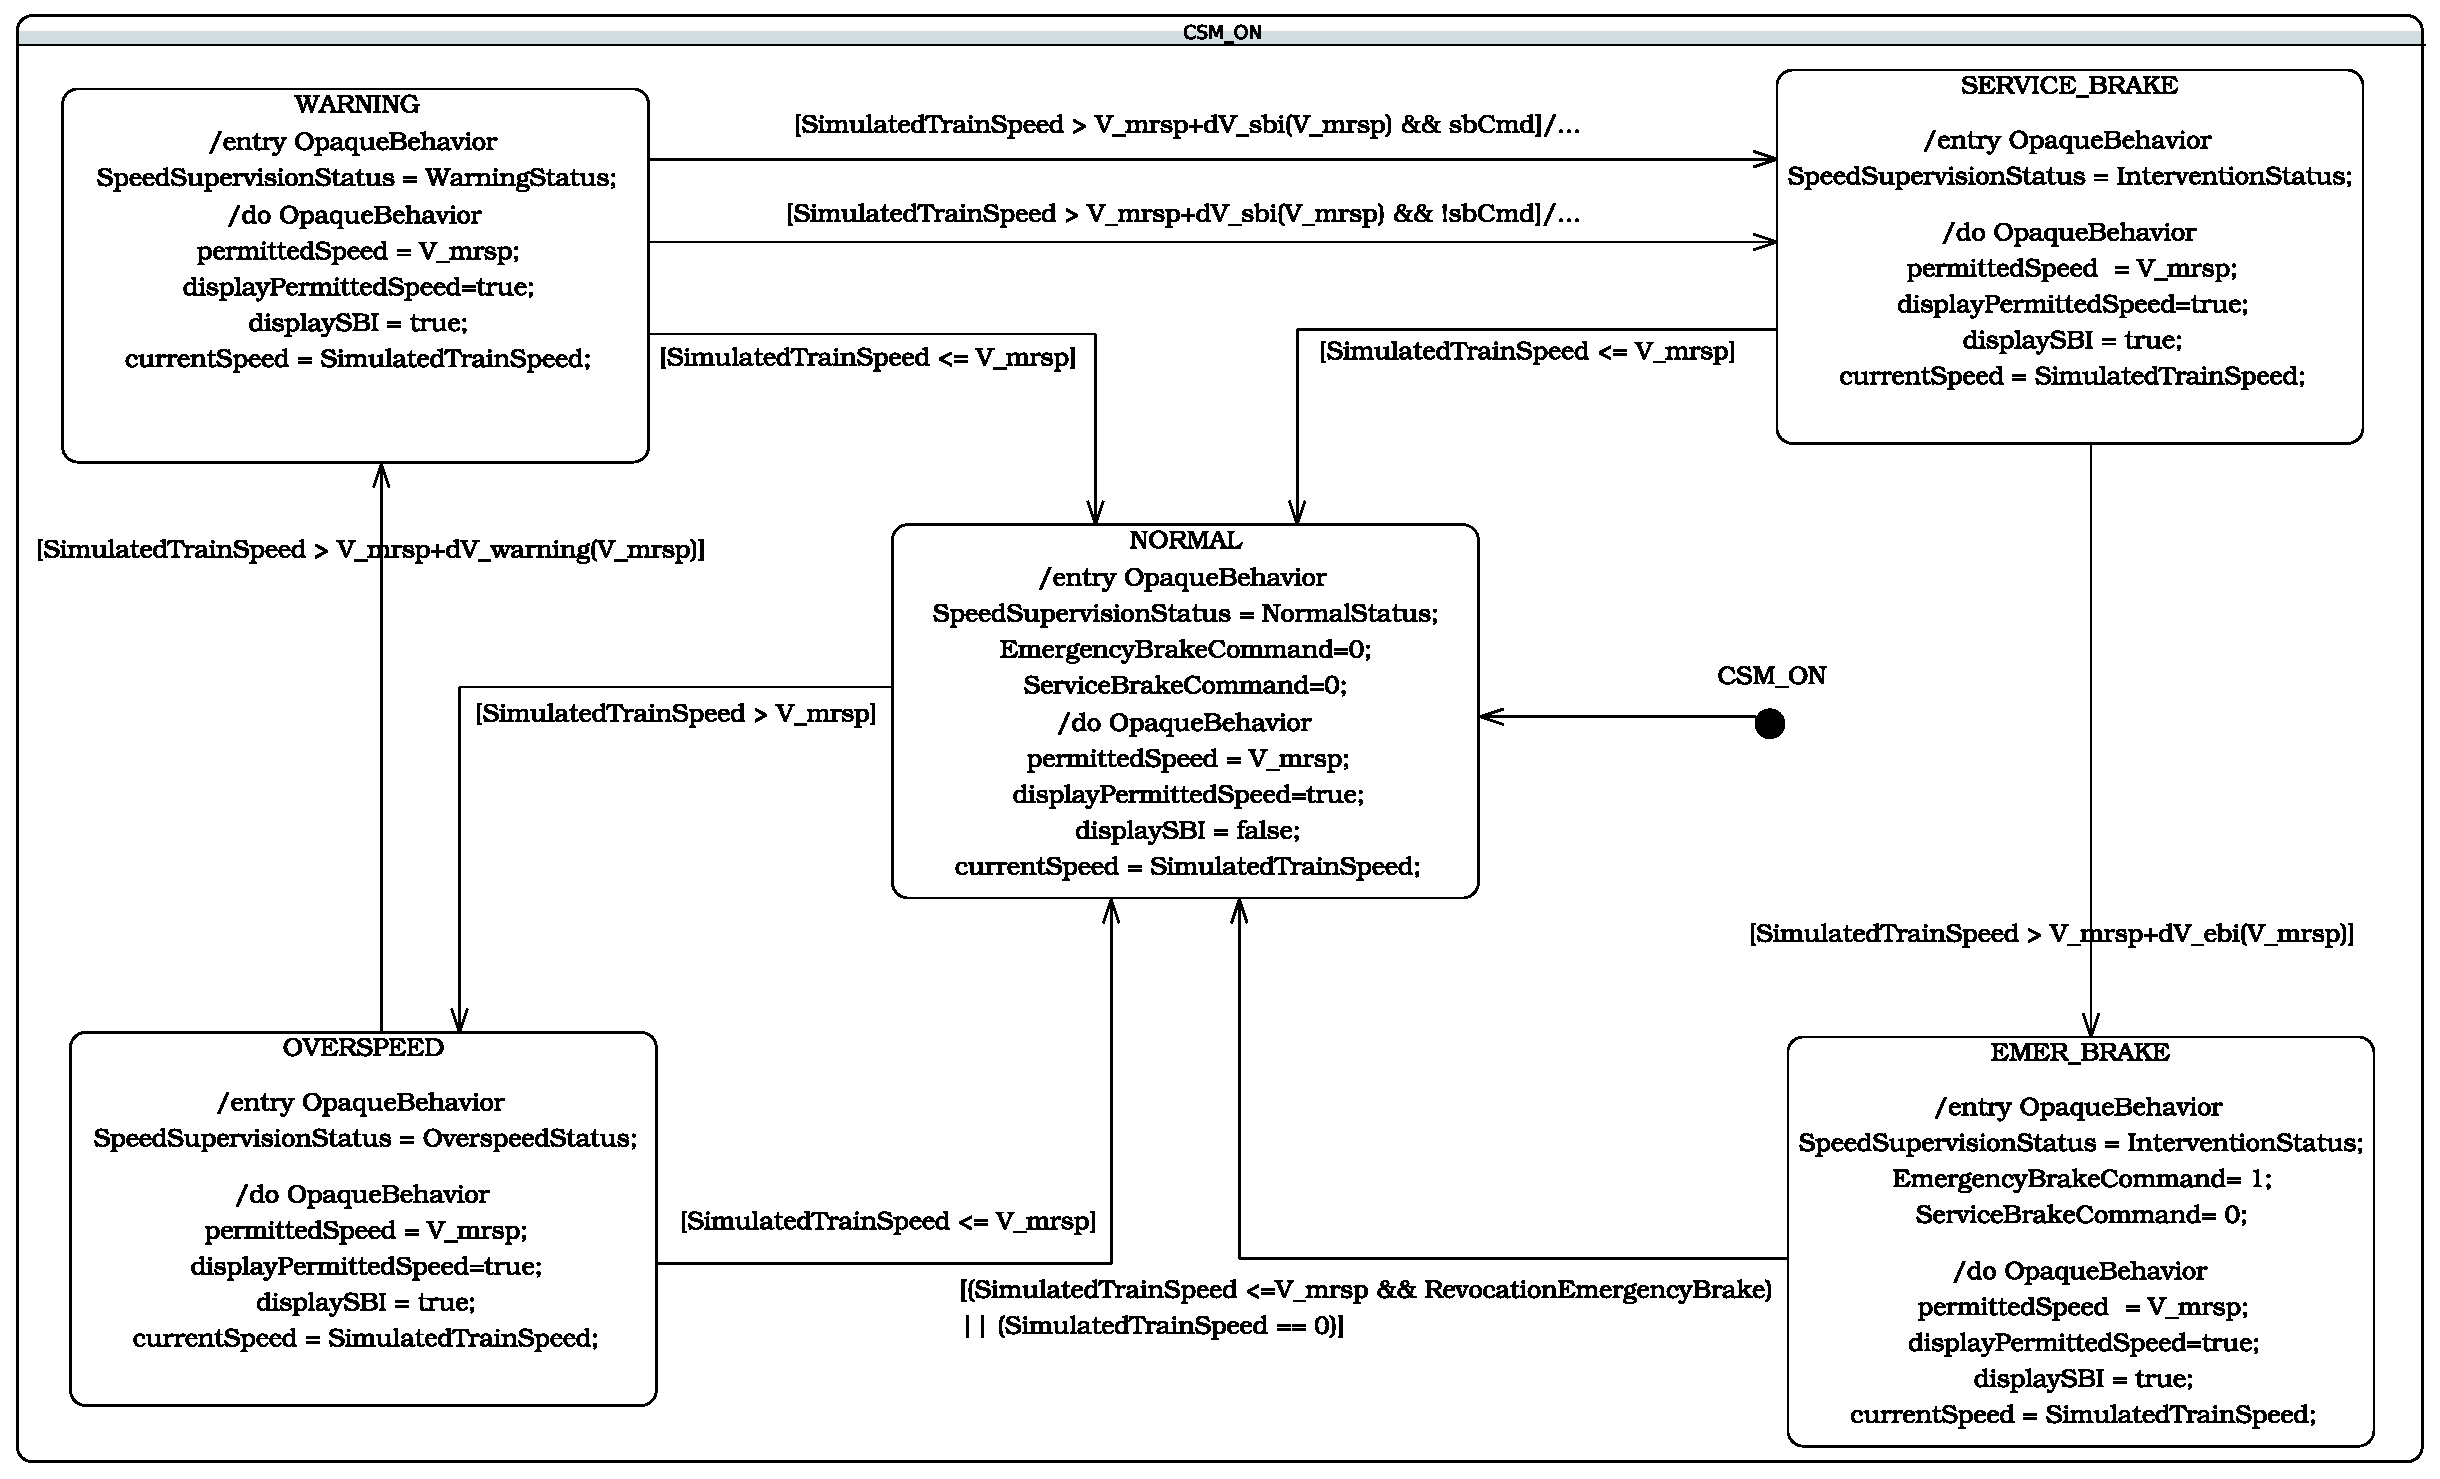
\includegraphics[width=\textwidth]{CSM-StateMachine.pdf}
%%\vspace*{-35mm}
\caption{Ceiling speed monitoring state machine.}
 \label{fig:csmsm}
 \end{figure}


Its execution starts in basic state {\sf NORMAL}, where the {\sf NormalStatus}
indication is displayed on the DMI and brakes are released 
($\ebcmd = 0$ and $\sbcmd = 0$). When the speed increases above the
maximal speed allowed ($\vest > \vmax$), the state machine transits to
basic state {\sf OVERSPEED}, where the {\sf OverspeedStatus} indication is displayed to the train engine driver. If the train continues over speeding until the warning threshold $\vmax + \dvw(\vmax)$ is exceeded, a transition
into the {\sf WARNING} state is performed, accompanied by an
indication change on the DMI. Accelerating further until $\vest >
\vmax + \dvs(\vmax)$ leads to a transition into basic state {\sf
  SERVICE\_BRAKE}, where either the service brake or the emergency
brake is triggered, depending on the value stored before in variable
$\sbicmd$. The DMI display changes to {\sf InterventionStatus}. 


 

The intervention status is realized by two basic state machine states, {\sf SERVICE\_BRAKE} and
{\sf EMER\_BRAKE}. From {\sf SERVICE\_BRAKE} it is still possible to return to {\sf NORMAL}, as soon as the speed has been decreased below the over speeding threshold. When the train, however, continues its acceleration until the emergency braking threshold has been exceeded ($\vest > \vmax+\dve(\vmax)$), basic state {\sf EMER\_BRAKE} is entered. From there, a state machine transition to {\sf NORMAL} is only possible if the train comes to a standstill, or if the national regulations (variable $\areb$)
allow to release the brakes as soon as over speeding has stopped.

Observe that the run-to-completion semantics of state machines also allows for zero-time
 transitions from, for example, {\sf NORMAL} to {\sf EMER\_BRAKE}. If,
 while in basic state {\sf NORMAL},  the inputs change such that
 $\vest > \vmax+\dve(\vmax)$ becomes true\footnote{This would be an
   exceptional behaviour situation, caused, for example, by temporary
   unavailability of odometry data, so that a ``sudden jump'' of
   $\vest$ would be observed by the CSM.}, the state machine
 transition from {\sf NORMAL} to {\sf OVERSPEED} leads to a transient
 model state, because guard condition $\vest > \vmax+\dvw(\vmax)$ is already
 fulfilled, and the state machine transits to {\sf
   WARNING}. Similarly, guards $\vest > \vmax+\dvs(\vmax)$ and $\vest >
 \vmax+\dve(\vmax)$ also evaluate to true, so that the next quiescent state
 is reached in basic state {\sf EMER\_BRAKE}.


% ============================================================
%%%@todo jp: add formal specification of the transition relation
% ============================================================

 



% .......................................................................
\subsection{Tracing Requirements to the Model}

SysML provides language elements for relating model elements to requirements, using the {\sf <<satisfy>>} relationship from model elements to requirements symbols in arbitrary SysML diagrams~\cite[Section~16]{SysML12}. Alternatively, SysML models may be augmented by
tables associating requirements and model elements. Exploiting this language feature supports both model validation and requirements-based testing.
In the former case, missing requirements can be detected if they
cannot be linked to structural or behavioural model elements in the
appropriate way. In latter case, execution traces through the model covering a
given structural or behavioural model element represent test cases
contributing to the verification of all requirements related to the
model element under consideration. 
%%%This technique is described in more detail below in Section~\ref{@todo}.
For the CSM model described above, the system requirements specified in 
Section~\ref{sec:sysreq} can be traced to model elements as follows.










\begin{table}[htbp]
\renewcommand{\arraystretch}{1.2}
\caption{Requirements links to the SysML
  Elements \label{table:req-tracing} }
\centering
\tabsize
\begin{tabular}{rrl}

\hline\hline
{\bf No.} & {\bf Requirement} & $\longleftarrow$ {\sf <<satisfy>>}
\\
\hline
1 &
REQ-3.13.10.2.1 & {\sf <<Composite State>>} {\sf CSM\_ON}  
\\\hline
2 &
REQ-3.13.10.2.2 & {\sf <<Transition>>} [{\sf EMER\_BRAKE} - {\sf NORMAL}]
\\ & &
{\sf <<Transition>>} [{\sf SERVICE\_BRAKE} - {\sf NORMAL}]
\\\hline
3 &
REQ-3.13.10.2.3 & {\sf <<Transition>>} [{\sf CSM\_OFF} - {\sf CSM\_ON}]
\\ & &
{\sf <<Basic State>>} {\sf SERVICE\_BRAKE}
\\ & &
{\sf <<Constraint>>} constraint\_03 
\\\hline
4 &
REQ-3.13.10.2.4 & {\sf <<Constraint>>} constraint\_02 
\\ & &
{\sf <<Transition>>} [{\sf EMER\_BRAKE} - {\sf NORMAL}]
\\ & &
{\sf <<Constraint>>} constraint\_01 
\\\hline
5 &
REQ-3.13.10.2.5 & {\sf <<Transition>>} [{\sf EMER\_BRAKE} - {\sf NORMAL}]
\\ & &
{\sf <<Transition>>} [{\sf SERVICE\_BRAKE} - {\sf NORMAL}]
\\\hline
6 &
REQ-3.13.10.3.1 & {\sf <<Submachine State>>} {\sf CSM\_ON}
\\\hline
7 &
REQ-3.13.10.3.2 & {\sf <<Basic State>>} {\sf OVERSPEED}  
\\ & &
{\sf <<Basic State>>} {\sf SERVICE\_BRAKE}  
\\ & &
{\sf <<Basic State>>} {\sf WARNING}  
\\ & &
{\sf <<Basic State>>} {\sf EMER\_BRAKE} 
\\\hline
8 &
REQ-3.13.10.3.3.r0 & {\sf <<Transition>>} [{\sf EMER\_BRAKE} - {\sf NORMAL}]
\\\hline
9 &
REQ-3.13.10.3.3.r1 & {\sf <<Transition>>} [{\sf OVERSPEED} - {\sf NORMAL}]
\\ & &
{\sf <<Transition>>} [{\sf SERVICE\_BRAKE} - {\sf NORMAL}]
\\ & &
{\sf <<Transition>>} [{\sf WARNING} - {\sf NORMAL}]
\\ & &
{\sf <<Transition>>} [{\sf EMER\_BRAKE} - {\sf NORMAL}]
\\\hline
10 &
REQ-3.13.10.3.3.t1 & {\sf <<Basic State>>} {\sf NORMAL}  
\\\hline
11 &
REQ-3.13.10.3.3.t2 & {\sf <<Basic State>>} {\sf OVERSPEED}  
\\\hline
12 &
REQ-3.13.10.3.3.t3 & {\sf <<Basic State>>} {\sf WARNING}  
\\\hline
13 &
REQ-3.13.10.3.3.t4 & {\sf <<Basic State>>} {\sf SERVICE\_BRAKE}  
\\\hline
14 &
REQ-3.13.10.3.3.t5 & {\sf <<Basic State>>} {\sf EMER\_BRAKE}  
\\\hline
15 &
REQ-3.13.10.3.4.r1c3 & {\sf <<Transition>>} [{\sf OVERSPEED} - {\sf NORMAL}]
\\\hline
16 &
REQ-3.13.10.3.4.r1c4 & {\sf <<Transition>>} [{\sf WARNING} - {\sf NORMAL}]
\\\hline
17 &
REQ-3.13.10.3.4.r1c5 & {\sf <<Transition>>} [{\sf EMER\_BRAKE} - {\sf NORMAL}]
\\ & &
{\sf <<Transition>>} [{\sf SERVICE\_BRAKE} - {\sf NORMAL}]
\\\hline
18 &
REQ-3.13.10.3.4.r3c1 & {\sf <<Transition>>} [{\sf NORMAL} - {\sf OVERSPEED}]
\\\hline
19 &
REQ-3.13.10.3.4.r4c1 & {\sf <<Constraint>>} constraint\_08 
\\\hline
20 &
REQ-3.13.10.3.4.r4c3 & {\sf <<Transition>>} [{\sf OVERSPEED} - {\sf WARNING}]
\\\hline
21 &
REQ-3.13.10.3.4.r5c1 & {\sf <<Constraint>>} constraint\_10 
\\ & &
{\sf <<Constraint>>} constraint\_09 
\\\hline
22 &
REQ-3.13.10.3.4.r5c3 & {\sf <<Constraint>>} constraint\_12 
\\ & &
{\sf <<Constraint>>} constraint\_11 
\\\hline
23 &
REQ-3.13.10.3.4.r5c4 & {\sf <<Transition>>} [{\sf WARNING} - {\sf SERVICE\_BRAKE}]
\\ & &
{\sf <<Transition>>} [{\sf SERVICE\_BRAKE} - {\sf EMER\_BRAKE}]
\\ & &
{\sf <<Constraint>>} constraint\_13 
\\\hline
24 &
REQ-3.13.10.3.5 & {\sf <<Constraint>>} constraint\_05 
\\ & &
{\sf <<Constraint>>} constraint\_06 
\\ & &
{\sf <<Constraint>>} constraint\_07 
\\ & &
{\sf <<Basic State>>} {\sf NORMAL} 
\\ & &
{\sf <<Constraint>>} constraint\_04 
\\\hline
25 &
REQ-3.13.10.3.6 & {\sf <<Constraint>>} constraint\_05 
\\ & &
{\sf <<Constraint>>} constraint\_06 
\\ & &
{\sf <<Constraint>>} constraint\_07 
\\ & &
{\sf <<Constraint>>} constraint\_04 

\\
\hline\hline
\end{tabular}

%%%@todo Modify run-to-completion/stability constraints

\end{table}


Tables \ref{table:req-tracing} associates 
the SysML elements with the requirements they satisfiy.  ``Submachine
State'' and  ``Atomic State'' refer to the top-level states of composite
machines and to basic control states, respectively. 
%% The ``Constraints" refer to
%% temporal logic formulas specified in LTL that are used to
%% relate the most complex requirements to execution traces as explained in Section~\ref{@todo}.
 

The complexity of {\sf <<satisfy>>} relations between structural or behavioural model elements depends on the complexity of the requirement and the way it is reflected by the structural and behavioural model. Consider, for example (see Table~\ref{tab:req}), requirement  
\begin{itemize}
\item REQ-3.13.10.2.1: The train speed indicated to the driver shall be identical to the speed used for the speed monitoring (i.e. the estimated speed $\vest$).
\end{itemize}

Every model trace where the CSM is activated is suitable for verifying this requirement, because the DMI variable $\std$ is updated by the actual speed $\vest$ via operation $\calcstd$, whenever the ceiling speed monitor is active, that is, in composite state {\sf CSM\_ON}. Therefore 
{\sf CSM\_ON} is linked to REQ-3.13.10.2.1 by the {\sf <<satisfy>>} relation, as expressed
in Table~\ref{table:req-tracing}, row~1. 

 


A more complex case of requirements tracing presents itself if one or more transitions are related to a given requirement. This is the case for the requirement
\begin{itemize}
\item REQ-3.13.10.2.2: Once a Train Interface command (traction cut-off, service brake or emergency brake) is triggered, the on-board shall apply it until its corresponding revocation condition is met.
\end{itemize}

As modeled in Fig.~\ref{fig:csmsm}, we have two revocation conditions; one is reflected by the transition from basic state {\sf SERVICE\_BRAKE} to {\sf NORMAL}, the other from {\sf EMER\_BRAKE} to {\sf NORMAL}. Therefore both transitions are related to REQ-3.13.10.2.2, as specified in row~2 of Table~\ref{table:req-tracing}.
In the  most complex case we have to handle situations where requirements are reflected by traces visiting model state {\it vectors}\footnote{A model state vector consists of valuations of  inputs, outputs, and internal model variables, as well as of variable valuations indicating the basic state machine states currently active.} fulfilling certain constraints, and these model state vectors have to be visited by the traces in a specific order. Such a situation is reflected, for example, by 
\begin{itemize}
\item REQ-3.13.10.3.4:
The on-board equipment shall execute the transitions between the different supervision statuses as described in Table~\ref{tab:seven} (see~\cite[4.6.1]{ETCSSRS-Principles} for details about the symbols). This table takes into account the order of precedence between the supervision statuses and the possible updates of the MRSP while in ceiling speed monitoring (e.g. when a TSR is revoked; TSR = Temporary Speed Restriction).
\end{itemize}


This requirement may be decomposed into atomic sub-requirements one
for each pertinent cells of table \ref{tab:six}.  Some of these
sub-requirements are again reflected by transitions. Sub-requirement
REQ-3.13.10.3.4.r5c1, however, specifies the possibility to directly
transit from {\sf NORMAL} to {\sf SERVICE\_BRAKE} or {\sf
  EMER\_BRAKE}. This cannot be specified by simply linking a
behavioural model element to the sub-requirement, because we have avoided
to draw direct state machine transitions from {\sf NORMAL} to {\sf
  SERVICE\_BRAKE} or {\sf EMER\_BRAKE}, since those transitions are
implicitly realized by the run-to-completion semantics, as explained
above. In the formalization of requirements tracing described in
Section~\ref{sec:formaltrc} we show how these situations can be
covered by using traceability specifications by means of temporal
logic formulas.
















